\documentclass[tikz,border=10pt]{standalone}
\usetikzlibrary{positioning}
\usepackage{tkz-graph}
\usepackage{rotating}

\usetikzlibrary{arrows}
%https://tex.stackexchange.com/questions/159127/drawing-simple-graph-pattern-with-tikz
\usetikzlibrary{arrows.meta}
\tikzset{main node/.style={circle,fill=blue!20,draw,minimum size=1cm,inner sep=0pt}}
\tikzset{simple node/.style={circle, fill=black,draw, inner sep=0pt,minimum size=5pt}}

\begin{document}

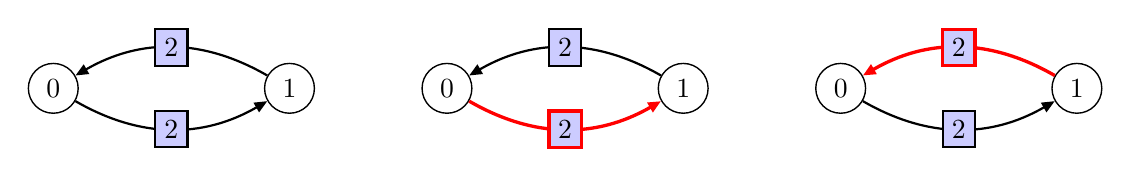
\begin{tikzpicture}
\SetGraphUnit{3}
\GraphInit[vstyle=Dijkstra]
\tikzset{EdgeStyle/.style = {-{Triangle[angle=45:5pt]},bend right,thick}}
\tikzset{LabelStyle/.style= {draw,fill = blue!20}}
\Vertex{0}
\EA(0){1}
\Edge[label=$2$](1)(0)
\Edge[label=$2$](0)(1)
\begin{scope}[xshift=5cm]
\SetGraphUnit{3}
\GraphInit[vstyle=Dijkstra]
\tikzset{EdgeStyle/.style = {-{Triangle[angle=45:5pt]},bend right,thick}}
\tikzset{LabelStyle/.style= {draw,fill=blue!20}}
\Vertex{0}
\EA(0){1}
\Edge[label=$2$](1)(0)
\SetUpEdge[style={draw=red,very thick,-{Triangle[angle=45:5pt]}, bend right}]
\tikzset{LabelStyle/.style ={draw,fill=blue!20}}
\Edge[label=$2$](0)(1)
\end{scope}
\begin{scope}[xshift=10cm]
\SetGraphUnit{3}
\GraphInit[vstyle=Dijkstra]
\tikzset{EdgeStyle/.style = {-{Triangle[angle=45:5pt]},bend right,thick}}
\tikzset{LabelStyle/.style= {draw,fill=blue!20}}
\Vertex{0}
\EA(0){1}
\Edge[label=$2$](0)(1)
\SetUpEdge[style={draw=red,very thick,-{Triangle[angle=45:5pt]}, bend right}]
\tikzset{LabelStyle/.style ={draw,fill=blue!20}}
\Edge[label=$2$](1)(0)
\end{scope}
\end{tikzpicture}


\end{document}